
\section{Abelian Anyon Vacuum on a Two-Handle Torus}
Using similar technique as in section 4.3, show that the ground state vacuum degeneracy on a two handle torus is $m^{2}$ for a system of abelian anyons with statistical angle $\theta =\pi p/m$ for integers $p$ and $m$ relatively prime. Hint: Consider what the independent nontrivial cycles are on a two-handled torus and determine the commutation relations for operators $T_{i}$ that take anyon-antianyon pairs around these cycles.

\paragraph{Answer}
There are four kinds of non-trivial loop in a genus-2 surface, as the Fig. \ref{fig:nontrivialLoopsOnTorus} below shows.
\begin{figure}[h!]
\centering
\tikzset {_j8ukpa9e3/.code = {\pgfsetadditionalshadetransform{ \pgftransformshift{\pgfpoint{0 bp } { 0 bp }  }  \pgftransformscale{1 }  }}}
\pgfdeclareradialshading{_ppijrrfvk}{\pgfpoint{0bp}{0bp}}{rgb(0bp)=(0.72,0.87,0.93);
rgb(0bp)=(0.72,0.87,0.93);
rgb(12.659355444567543bp)=(0.13,0.71,0.89);
rgb(25bp)=(0.72,0.87,0.93);
rgb(400bp)=(0.72,0.87,0.93)}
\tikzset{_h64hwuq6d/.code = {\pgfsetadditionalshadetransform{\pgftransformshift{\pgfpoint{0 bp } { 0 bp }  }  \pgftransformscale{1 } }}}
\pgfdeclareradialshading{_dg2f1u1o5} { \pgfpoint{0bp} {0bp}} {color(0bp)=(transparent!0);
color(0bp)=(transparent!0);
color(12.659355444567543bp)=(transparent!41);
color(25bp)=(transparent!0);
color(400bp)=(transparent!0)} 
\pgfdeclarefading{_suy8hqhn4}{\tikz \fill[shading=_dg2f1u1o5,_h64hwuq6d] (0,0) rectangle (50bp,50bp); } 

% Gradient Info
  
\tikzset {_pa6e1atmm/.code = {\pgfsetadditionalshadetransform{ \pgftransformshift{\pgfpoint{0 bp } { 0 bp }  }  \pgftransformscale{1 }  }}}
\pgfdeclareradialshading{_kdcnmoyz0}{\pgfpoint{0bp}{0bp}}{rgb(0bp)=(0.72,0.87,0.93);
rgb(0bp)=(0.72,0.87,0.93);
rgb(12.659355444567543bp)=(0.13,0.71,0.89);
rgb(25bp)=(0.72,0.87,0.93);
rgb(400bp)=(0.72,0.87,0.93)}
\tikzset{_dbhaxkn5n/.code = {\pgfsetadditionalshadetransform{\pgftransformshift{\pgfpoint{0 bp } { 0 bp }  }  \pgftransformscale{1 } }}}
\pgfdeclareradialshading{_3ijpfagau} { \pgfpoint{0bp} {0bp}} {color(0bp)=(transparent!0);
color(0bp)=(transparent!0);
color(12.659355444567543bp)=(transparent!41);
color(25bp)=(transparent!0);
color(400bp)=(transparent!0)} 
\pgfdeclarefading{_1alqmfhm2}{\tikz \fill[shading=_3ijpfagau,_dbhaxkn5n] (0,0) rectangle (50bp,50bp); } 

% Gradient Info
  
\tikzset {_39sy1qdqi/.code = {\pgfsetadditionalshadetransform{ \pgftransformshift{\pgfpoint{0 bp } { 0 bp }  }  \pgftransformrotate{0 }  \pgftransformscale{2 }  }}}
\pgfdeclarehorizontalshading{_2iq1vrbsa}{150bp}{rgb(0bp)=(0.44,0.81,0.95);
rgb(37.5bp)=(0.44,0.81,0.95);
rgb(49.82457216296877bp)=(0.44,0.81,0.94);
rgb(62.5bp)=(0.58,0.84,0.94);
rgb(100bp)=(0.58,0.84,0.94)}
\tikzset{_jx9sr6k5x/.code = {\pgfsetadditionalshadetransform{\pgftransformshift{\pgfpoint{0 bp } { 0 bp }  }  \pgftransformrotate{0 }  \pgftransformscale{2 } }}}
\pgfdeclarehorizontalshading{_vwzi310up} {150bp} {color(0bp)=(transparent!25);
color(37.5bp)=(transparent!25);
color(49.82457216296877bp)=(transparent!69);
color(62.5bp)=(transparent!32);
color(100bp)=(transparent!32) } 
\pgfdeclarefading{_2j9mzfwq8}{\tikz \fill[shading=_vwzi310up,_jx9sr6k5x] (0,0) rectangle (50bp,50bp); } 
\tikzset{every picture/.style={line width=0.75pt}} %set default line width to 0.75pt        

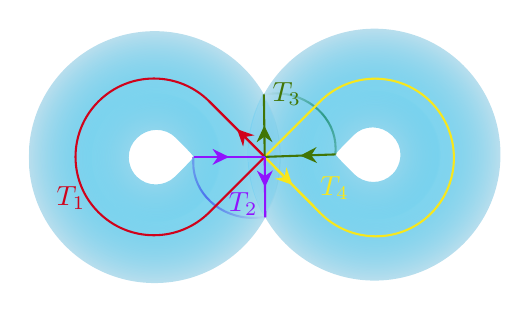
\begin{tikzpicture}[x=0.75pt,y=0.75pt,yscale=-1,xscale=1]
%uncomment if require: \path (0,131); %set diagram left start at 0, and has height of 131

%Shape: Arc [id:dp680359352005554] 
\draw  [draw opacity=0] (331.52,96.03) .. controls (329.78,96.33) and (327.98,96.48) .. (326.15,96.48) .. controls (310.2,96.48) and (297.27,84.6) .. (297.27,69.93) .. controls (297.27,68.97) and (297.32,68.02) .. (297.43,67.09) -- (326.15,69.93) -- cycle ; \draw  [color={rgb, 255:red, 144; green, 19; blue, 254 }  ,draw opacity=1 ] (331.52,96.03) .. controls (329.78,96.33) and (327.98,96.48) .. (326.15,96.48) .. controls (310.2,96.48) and (297.27,84.6) .. (297.27,69.93) .. controls (297.27,68.97) and (297.32,68.02) .. (297.43,67.09) ;  
%Shape: Arc [id:dp3309974302317926] 
\draw  [draw opacity=0] (331.63,36.96) .. controls (333.37,36.66) and (335.17,36.5) .. (337,36.5) .. controls (352.95,36.5) and (365.88,48.39) .. (365.88,63.05) .. controls (365.88,64.02) and (365.83,64.97) .. (365.72,65.9) -- (337,63.05) -- cycle ; \draw  [color={rgb, 255:red, 65; green, 117; blue, 5 }  ,draw opacity=1 ] (331.63,36.96) .. controls (333.37,36.66) and (335.17,36.5) .. (337,36.5) .. controls (352.95,36.5) and (365.88,48.39) .. (365.88,63.05) .. controls (365.88,64.02) and (365.83,64.97) .. (365.72,65.9) ;  
%Shape: Path Data [id:dp5162766569900514] 
\draw  [draw opacity=0][shading=_ppijrrfvk,_j8ukpa9e3,path fading= _suy8hqhn4 ,fading transform={xshift=2}] (278.7,6.53) .. controls (312.21,6.53) and (339.38,33.69) .. (339.38,67.21) .. controls (339.38,100.72) and (312.21,127.88) .. (278.7,127.88) .. controls (245.19,127.88) and (218.02,100.72) .. (218.02,67.21) .. controls (218.02,33.69) and (245.19,6.53) .. (278.7,6.53) -- cycle (266.2,67.21) .. controls (266.2,68.48) and (266.39,69.71) .. (266.74,70.87) .. controls (267.31,72.97) and (268.42,74.96) .. (270.06,76.6) .. controls (275.16,81.69) and (283.48,81.63) .. (288.66,76.45) .. controls (294.71,70.41) and (297.63,67.29) .. (297.43,67.09) .. controls (297.63,66.89) and (294.76,63.81) .. (288.81,57.86) .. controls (283.71,52.77) and (275.39,52.83) .. (270.21,58.01) .. controls (270.14,58.08) and (270.07,58.15) .. (270.01,58.22) .. controls (267.66,60.49) and (266.2,63.68) .. (266.2,67.21) -- cycle ;
%Shape: Path Data [id:dp03607295158679058] 
\draw  [draw opacity=0][shading=_kdcnmoyz0,_pa6e1atmm,path fading= _1alqmfhm2 ,fading transform={xshift=2}] (384.61,5.34) .. controls (351.1,5.34) and (323.93,32.5) .. (323.93,66.02) .. controls (323.93,99.53) and (351.1,126.69) .. (384.61,126.69) .. controls (418.12,126.69) and (445.29,99.53) .. (445.29,66.02) .. controls (445.29,32.5) and (418.12,5.34) .. (384.61,5.34) -- cycle (397.11,66.02) .. controls (397.11,67.29) and (396.92,68.52) .. (396.57,69.68) .. controls (396,71.78) and (394.89,73.77) .. (393.25,75.41) .. controls (388.15,80.5) and (379.83,80.44) .. (374.65,75.26) .. controls (368.61,69.22) and (365.69,66.1) .. (365.88,65.9) .. controls (365.68,65.7) and (368.56,62.62) .. (374.51,56.67) .. controls (379.6,51.58) and (387.92,51.64) .. (393.1,56.82) .. controls (393.17,56.89) and (393.24,56.96) .. (393.31,57.03) .. controls (395.65,59.3) and (397.11,62.49) .. (397.11,66.02) -- cycle ;
%Shape: Path Data [id:dp07597847208253206] 
\draw  [draw opacity=0][shading=_2iq1vrbsa,_39sy1qdqi,path fading= _2j9mzfwq8 ,fading transform={xshift=2}] (338.91,66.98) .. controls (338.91,77.5) and (336.23,87.4) .. (331.52,96.03) .. controls (326.39,87.12) and (323.46,76.8) .. (323.46,65.79) .. controls (323.46,55.27) and (326.14,45.37) .. (330.85,36.74) .. controls (335.98,45.65) and (338.91,55.97) .. (338.91,66.98) -- cycle ;
%Shape: Tear Drop [id:dp23567666397505516] 
\draw  [color={rgb, 255:red, 208; green, 2; blue, 27 }  ,draw opacity=1 ] (305.03,93.79) .. controls (305.03,93.79) and (305.03,93.79) .. (305.03,93.79) .. controls (290.28,108.53) and (266.37,108.53) .. (251.63,93.79) .. controls (236.88,79.04) and (236.88,55.14) .. (251.63,40.39) .. controls (266.37,25.65) and (290.28,25.65) .. (305.03,40.39) .. controls (322.83,58.19) and (331.72,67.08) .. (331.72,67.09) .. controls (331.72,67.08) and (322.82,75.99) .. (305.03,93.79) -- cycle ;
%Shape: Tear Drop [id:dp6795678748133291] 
\draw  [color={rgb, 255:red, 248; green, 231; blue, 28 }  ,draw opacity=1 ] (358.42,94.09) .. controls (358.42,94.09) and (358.42,94.09) .. (358.42,94.09) .. controls (373.16,109) and (397.07,109.13) .. (411.82,94.38) .. controls (426.56,79.64) and (426.56,55.6) .. (411.82,40.69) .. controls (397.07,25.78) and (373.17,25.64) .. (358.42,40.39) .. controls (340.62,58.19) and (331.72,67.09) .. (331.72,67.09) .. controls (331.72,67.09) and (340.62,76.09) .. (358.42,94.09) -- cycle ;
%Straight Lines [id:da3250412655048094] 
\draw [color={rgb, 255:red, 208; green, 2; blue, 27 }  ,draw opacity=1 ]   (305.03,40.39) -- (331.72,67.09) ;
\draw [shift={(318.37,53.74)}, rotate = 45] [fill={rgb, 255:red, 208; green, 2; blue, 27 }  ,fill opacity=1 ][line width=0.08]  [draw opacity=0] (8.04,-3.86) -- (0,0) -- (8.04,3.86) -- (5.34,0) -- cycle    ;
%Straight Lines [id:da7533241799472672] 
\draw [color={rgb, 255:red, 248; green, 231; blue, 28 }  ,draw opacity=1 ]   (358.42,94.09) -- (331.72,67.09) ;
\draw [shift={(345.07,80.59)}, rotate = 225.32] [fill={rgb, 255:red, 248; green, 231; blue, 28 }  ,fill opacity=1 ][line width=0.08]  [draw opacity=0] (8.04,-3.86) -- (0,0) -- (8.04,3.86) -- (5.34,0) -- cycle    ;
%Straight Lines [id:da0896284008005579] 
\draw [color={rgb, 255:red, 65; green, 117; blue, 5 }  ,draw opacity=1 ]   (331.32,36.97) -- (331.72,67.09) ;
\draw [shift={(331.52,52.03)}, rotate = 89.24] [fill={rgb, 255:red, 65; green, 117; blue, 5 }  ,fill opacity=1 ][line width=0.08]  [draw opacity=0] (8.04,-3.86) -- (0,0) -- (8.04,3.86) -- (5.34,0) -- cycle    ;
%Straight Lines [id:da46999426860174665] 
\draw [color={rgb, 255:red, 65; green, 117; blue, 5 }  ,draw opacity=1 ]   (365.88,65.9) -- (331.72,67.09) ;
\draw [shift={(348.8,66.49)}, rotate = 358] [fill={rgb, 255:red, 65; green, 117; blue, 5 }  ,fill opacity=1 ][line width=0.08]  [draw opacity=0] (8.04,-3.86) -- (0,0) -- (8.04,3.86) -- (5.34,0) -- cycle    ;
%Straight Lines [id:da30598677739448976] 
\draw [color={rgb, 255:red, 144; green, 19; blue, 254 }  ,draw opacity=1 ]   (331.99,96.25) -- (331.72,67.09) ;
\draw [shift={(331.86,81.67)}, rotate = 269.48] [fill={rgb, 255:red, 144; green, 19; blue, 254 }  ,fill opacity=1 ][line width=0.08]  [draw opacity=0] (8.04,-3.86) -- (0,0) -- (8.04,3.86) -- (5.34,0) -- cycle    ;
%Straight Lines [id:da9986296639008827] 
\draw [color={rgb, 255:red, 144; green, 19; blue, 254 }  ,draw opacity=1 ]   (331.72,67.09) -- (297.43,67.09) ;
\draw [shift={(314.58,67.09)}, rotate = 180.01] [fill={rgb, 255:red, 144; green, 19; blue, 254 }  ,fill opacity=1 ][line width=0.08]  [draw opacity=0] (8.04,-3.86) -- (0,0) -- (8.04,3.86) -- (5.34,0) -- cycle    ;


% Text Node
\draw (230,79.93) node [anchor=north west][inner sep=0.75pt]  [color={rgb, 255:red, 208; green, 2; blue, 27 }  ,opacity=1 ]  {$T_{1}$};
% Text Node
\draw (313,82.93) node [anchor=north west][inner sep=0.75pt]  [color={rgb, 255:red, 144; green, 19; blue, 254 }  ,opacity=1 ]  {$T_{2}$};
% Text Node
\draw (334,29.93) node [anchor=north west][inner sep=0.75pt]  [color={rgb, 255:red, 65; green, 117; blue, 5 }  ,opacity=1 ]  {$T_{3}$};
% Text Node
\draw (357,74.93) node [anchor=north west][inner sep=0.75pt]  [color={rgb, 255:red, 248; green, 231; blue, 28 }  ,opacity=1 ]  {$T_{4}$};
\end{tikzpicture}
\caption{Nontrivial loops on genus-2 surface.}
\label{fig:nontrivialLoopsOnTorus}
\end{figure}

This time, we cannot use only one complex number to label the state, since $T_{1}$ and $T_{4}$ don't commute. We call
\begin{equation*}
T_{1} |\alpha ,\beta \rangle =\mathrm{e}^{\mathrm{i} \alpha } |\alpha ,\beta \rangle ;\quad T_{4}\ket{\alpha ,\beta } =\mathrm{e}^{\mathrm{i} \beta } |\alpha ,\beta \rangle .
\end{equation*}
Now we can repeat the same deduction in section 4.3. The commutator gives
\begin{equation*}
T_{2} T_{1} =\mathrm{e}^{-2\mathrm{i} \theta } T_{1} T_{2} ;\quad T_{3} T_{4} =\mathrm{e}^{-2\mathrm{i} \theta } T_{4} T_{3}
\end{equation*}
and
\begin{equation*}
\begin{aligned}
T_{1}( T_{2} |\alpha ,\beta \rangle ) & =\mathrm{e}^{2\mathrm{i} \theta } T_{2} T_{1}\ket{\alpha ,\beta } =\mathrm{e}^{2\mathrm{i} \theta }\mathrm{e}^{\mathrm{i} \alpha }( T_{2} |\alpha ,\beta \rangle )\\
T_{4}( T_{3} |\alpha ,\beta \rangle ) & =\mathrm{e}^{2\mathrm{i} \theta } T_{3} T_{4}\ket{\alpha ,\beta } =\mathrm{e}^{2\mathrm{i} \theta }\mathrm{e}^{\mathrm{i} \beta }( T_{3} |\alpha ,\beta \rangle ) .
\end{aligned}
\end{equation*}
Now, for $T_{2}$ we have $m$ basis states:
\begin{equation*}
|\alpha ,\beta \rangle ,|\alpha +2\pi p/m,\beta \rangle ,\cdots ,|\alpha +2\pi ( m-1) p/m,\beta \rangle .
\end{equation*}
However, this time, each state of these is a new "generator" for $T_{3}$, for example
\begin{equation*}
|\alpha +2\pi p/m,\beta \rangle \rightarrow |\alpha +2\pi p/m,\beta +2\pi p/m\rangle \rightarrow \cdots \rightarrow |\alpha +2\pi p/m,\beta +2\pi ( m-1) p/m\rangle .
\end{equation*}
So there are totally $m^{2}$ basis states for a genus $2$ surface. For genus $g$ surface, the GSD is $m^{g}$. 
